\section{Theroritical Background}
\subsection{QD 'Artificial Atoms'}
Self-assembled quantum dots (QDs) are localized nano-scale semiconductor structures that creates a three-dimensional(3D) potential well, both in the valence and conduction bands,which trap charge carriers. Due to their small confinement length relative to the particle's wavelength, the energy levels of the QD are quantized with properties similar to atoms which lead them to be described as "Artificial Atoms" \cite{Kastner1993}. \\
In recent years, semiconductor QDs were thoroughly investigated as technology-compatible single photon sources, providing a quantum source of "flying qubits" on demand.\cite{Dekel2000,Michler2000,Michler2000_1,Yuan2002} Moreover, recently, it has been shown that QDs can emit pair of entangled photons \cite{Akopian2006,Hafenbrak2007} and that an emitted photon can be entangled with the remaining spin in the QD. \cite{Pelk2012,Schaibley2013,Gao2012} These achievements form the required building blocks for quantum information processing. \cite{DiVincenzo1998,Duan2001}\\
\subsection{Entangled photons}
\subsubsection{Definition of Entanglement}
Quantum entanglement is a phenomenon in quantum mechanics where two or more particles can become correlated in such a way that the state of each particle cannot be described independently of the state of the others. 
 In other words, The overall state cannot be expressed as a product of the states of their subsystems. In other words, an entangled system is not separable.\\
 If, on the other hand, the system is prepared in a separable state, then the overall state can be expressed as a product of the states of the individual particles. In this case, the particles are not entangled, and their states can be described independently of each other.
\subsubsection{The role of entangled photon s in quantum information}
Entanglement is a crucial resource in quantum information processing, enabling key advantages over classical information processing and making possible many of the most exciting and promising applications of quantum technologies.
\paragraph{Quantum communication}
Quantum communication is all about transferring a quantum state from one place to the other. Entanglement has a big role in doing that. Entanglement between light and matter is used to perform quantum state transfer and entanglement distribution among distant nodes.  Cirac [10] suggested a protocol in which atoms in a cavity are excited by a laser, mapping the atom state to a photon wave packet that enters a cavity at the receiving node. Quantum repeaters [11] correct errors in an entanglement that increase with distance and transmit entangled quantum states over large distances.
\subsubsection{Fundamental excitations in QD}
In semiconductor QDs, at low temperatures, the basic optical excitation, in which an electron is optically excited from the full valence band, thereby leaving there a hole, to the empty conduction band, is called a bright exciton(BE). In self-assembled QDs, the BE consists of an electron-heavy-hole pair. This optical excitation preserves the excited electron's spin orientation; therefore, the electron and hole have anti-parallel spins. The total angular momentum projection of the BE in the direction of the exciting light is ±1 (like that of the absorbed photon), reflecting the orbital momentum difference between the electron in the valence band to that in the conduction band.
If the excited conduction electron's spin projection is in addition opposite to the spin projection of the ground valence band electron, the electron, and the 2 holes have parallel spins, with a total angular momentum projection of ±2. This type of excitation is optically forbidden since the light electric field cannot change the electronic spin; therefore, it is called dark exciton (DE). Excitons in the QD can also be generated while the QD contains additional charges, such as a single electron or a single hole. Similarly, many other types of multiple carrier configurations can populate the QD simultaneously. For example, a biexciton is two excitons (two electrons and two holes), and a positively (negatively) charged exciton (trion) is an exciton with the addition of one hole (electron) 
\subsubsection{The $\Lambda$ and $\Pi$ systems}
$\Lambda$ system is a three-level physical system in which the two eigenstates of a qubit are connected to a third auxiliary level via an optical transition. An example of a relevant to this proposal Λ system is presented in Figure $\ref{fig:PiSystem}$(a), where the two (degenerate) BE eigenstates are coupled to the ground (nondegenerate) biexciton state. Similarly, one can also think about the BE and the (non-degenerate) vacuum level as an Inverted Λ system or a V system (not shown). 
\begin{figure}[H]
	\centering
	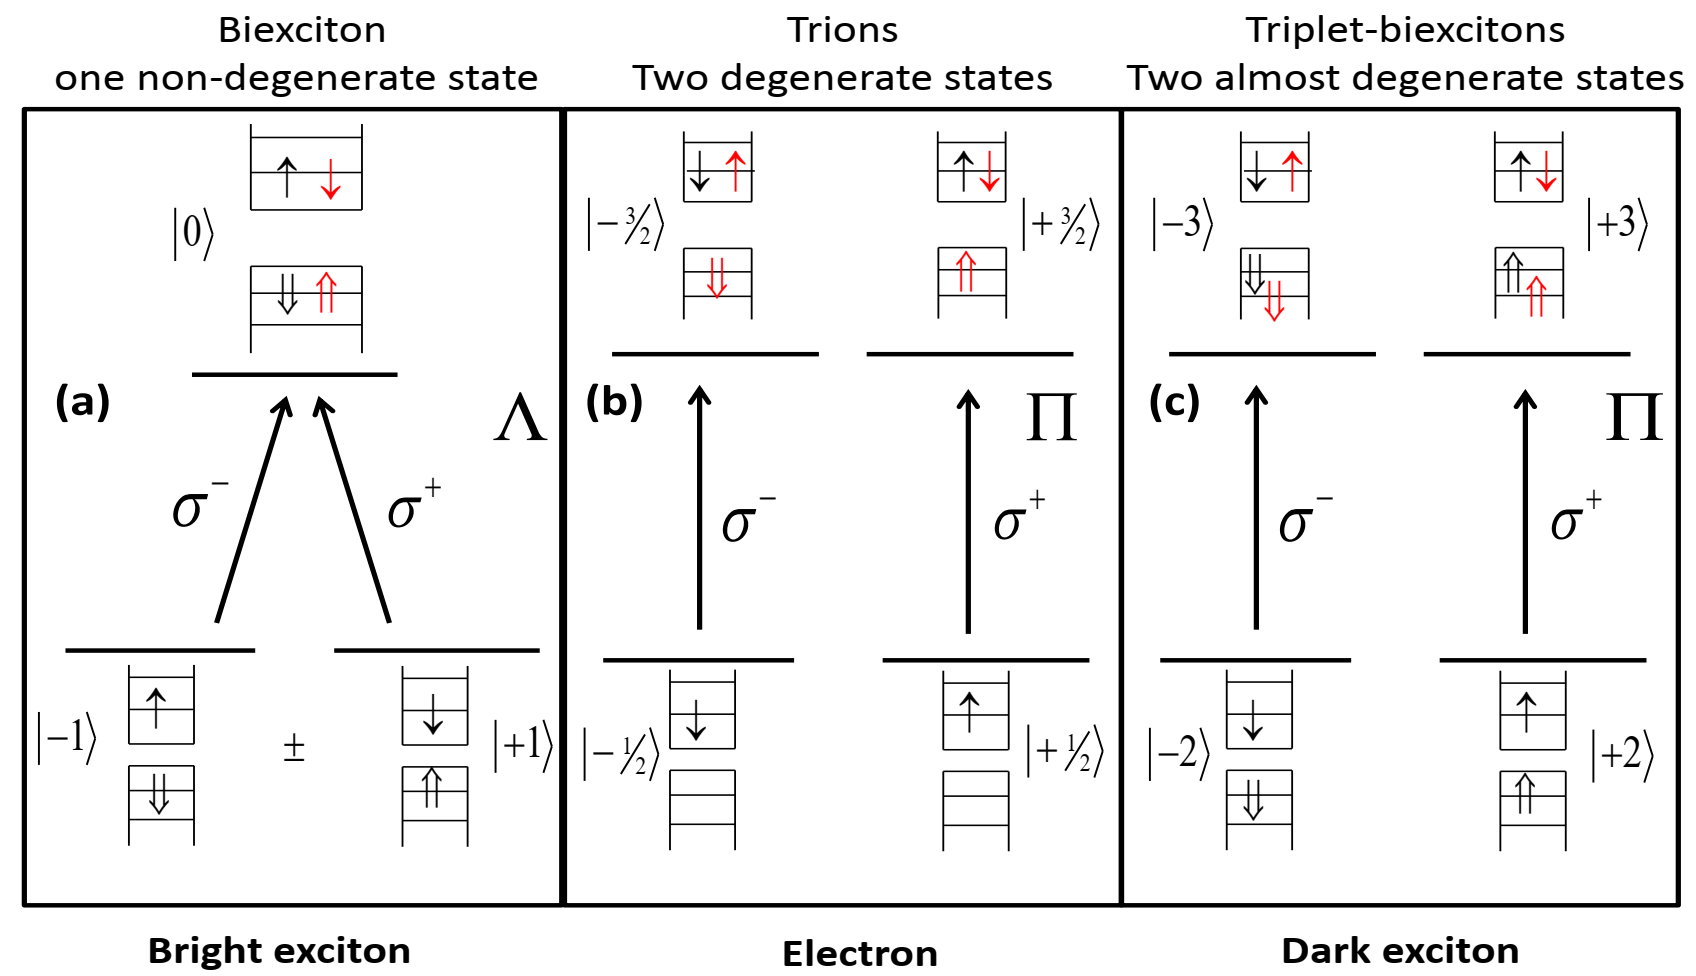
\includegraphics[scale=0.32]{figures/pISystem.png}
	\caption{Schematic description of the energy level and selection rules for
optical transition in Λ and Π systems. (a) The BE and the ground biexciton form a $\Lambda$ system. (b) A (degenerate) electron spin forms a $\Pi$ qubit system
with the excited trion states. (c) The (degenerate) DE forms a Π qubit system
with the excited biexciton state. The states are described by their total
angular momentum projections. The arrows symbolize optical transitions, and σ+ (σ-) symbolizes right (left) hand circular polarization.}
	\label{fig:PiSystem}
\end{figure}
A Λ system has physical properties which are very useful for QIP. Notably,
since the radiative decay of the non-degenerate auxiliary level to the qubit has
two paths, the lack of "which-path" information leads to entanglement
between the emitted photon polarization and the remaining matter qubit
spin. This kind of entanglement between a photon and matter spin qubit – the
exciton was first demonstrated by Akopian et al
\subsubsection{QD as a source of single photon}
\subsubsection{exciton-biexciton cascade (QD as a source of entangled photon pair)}
The projection of the spin of the electron on the z-axis (growth axis) of the QD can be either 1/2 or -1/2, while for the heavy hole, the spin 
 projection is either 3/2 or -3/2 such that the two spin states of the bright exciton are $\ket{\frac{1}{2},-\frac{2}{3}}$ and $\ket{-\frac{1}
 {2},\frac{2}{3}}$  with a total spin in the z direction  of $\pm1$. While in the case of electron-hole pair with parallel spin, the spin states are $\ket{\frac{1}{2},\frac{2}{3}}$ and $\ket{-\frac{1}{2},-\frac{2}{3}}$ with a total spin of $\pm2$.\\
	In figure \ref{fig:energy_levels}, we describe two simple configurations we can have in a QD. We start with an empty dot denoted by $\ket{0}$.
	\begin{figure}[H]
		\centering
		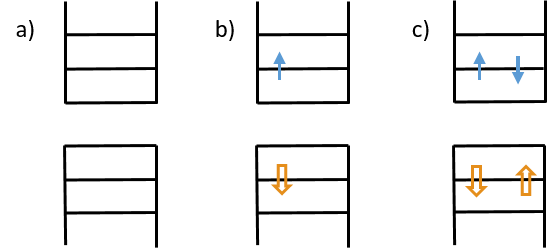
\includegraphics[scale=1]{figures/energy-levels.png}
		\caption{Schematic of the energy levels in the quantum dot for empty quantum dot (a), exciton (b), and a biexciton (c)}
		\label{fig:energy_levels}
	\end{figure}
	while having two electron-hole pairs falling in the dot, a biexciton is formed, and we denote it by $\ket{{XX}_0}$. The total energy of the biexciton differs from twice the energy of the exciton due to the interaction between all the particles.\\
	In an ideal QD, the radiative decay path of the biexciton back to the ground state goes via one path. But due to the anisotropy of the QD, the energy of exciton is split in what is defined as the fine structure splitting (FSS) as seen in figure \ref{fig:figureDecay_paths}b. Here we refer to the up (down) spin of the electron as $\ket{\uparrow}$ ($\ket{\downarrow}$ and the up (down) spin of the hole as $\ket{\Uparrow}$ ($\ket{\Downarrow}$ such as the two eigenstates of the exciton are  $\ket{\uparrow\Downarrow}$ and $\ket{\downarrow\Uparrow}$, and the decay from these states result in the emission of photons with co-linear polarization. Here we refer to them as horizontal $\ket{H}$ and vertical $\ket{V}$. We can represent these two rectilinear bases using the Bloch sphere, where the poles in the sphere are $\ket{H}$ and $\ket{V}$ bases.\\
	
	In addition to the rectilinear polarization states, We can define the diagonal linear and
	the circular polarization bases: 
	\begin{equation}
		\begin{split}
			\ket{L}=(\ket{H}+i\ket{V})/\sqrt{2} \\
			\ket{R}=(\ket{H}-i\ket{V})/\sqrt{2}
		\end{split}
	\end{equation}
	Where $\ket{R}$ and $\ket{L}$ are the left and right circular bases, respectively, and:
	\begin{equation}
		\begin{split}
			\ket{D}=(\ket{H}+\ket{V})/\sqrt{2}\\
			\ket{\bar{D}}=(\ket{H}+\ket{V})/\sqrt{2}
		\end{split}
	\end{equation}
	$\ket{D}$ and $\ket{\bar{D}}$ are the diagonal and anti-diagonal bases respectively
	
	\begin{figure}[H]
		a)
		\raggedleft
		\def\psiLat{0}
		\def\psiLon{-50}
		\begin{blochsphere}[radius=2.5 cm,tilt=20,rotation=-20,opacity=0]
			\labelLatLon{psi}{\psiLat}{-\psiLon};
			\draw[-latex] (0,0) -- (psi) node[above]{$\large\ket{\psi}$};
			\drawRotationLeft[scale=0.9,style={red}]{0}{0}{0}{15}
			
			\drawGreatCircle[style={dashed}]{0}{0}{0}
			\drawBallGrid[style={opacity=0.5}]{30}{30}
			\draw [fill] (0,0) circle (1.5pt);
			\drawGreatCircle[style={dashed}]{0}{0}{0}
			\labelLatLon{up}{90}{0};
			\labelLatLon{down}{-90}{90};
			\node[above] at (up) {{ $\ket{H}$ }};
			\node[below] at (down) {{ $\ket{V}$}};
			\node at (2.8,0) {{$\ket{R}$}};
			\node at (-2.8,0) {{$\ket{L}$}};
			\node at (0,1) {{$\ket{D}$}};
			\node at (0,-1) {{$\ket{\bar{D}}$}};
		\end{blochsphere}
		b)
		\raggedright
		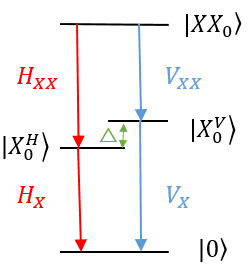
\includegraphics[scale=0.8]{figures/Decay_paths.png}
		\caption{a) A Bloch sphere representation of the spin state. A point on the sphere represents an arbitrarily polarized spin state. b) Decay paths of the biexciton back to the ground state where the red arrows represent the emission of an H-polarized photon and the blue arrows represent the emission of a V-polarized photon.}
		\label{fig:Decay_paths}
	\end{figure}
	When the biexciton spontaneously radiatively decays, it  emits a photon leaving 
	in the QD, an exciton in a coherent superposition of its two eigenstates. The optical
	selection rules for the biexciton radiative recombination and the lack of information by “which path” the recombination proceeds result in the entanglement between the exciton state and the polarization state of the emitted photon. Their mutual wave function is given by:
	\begin{equation}
		\ket{\psi_{X^0}} = \frac{1}{\sqrt{2}}(\ket{H_1H^1_H} +\ket{V_1V^1_V})
	\end{equation}
	here $\ket{H_1}$ and $\ket{V1}$ are the two rectilinear polarization states of the first (biexciton) photon. Since the two exciton eigenstates are not degenerate, the relative phase between these eigenstates precesses in time with a period of $T_P = h/\triangle$, where $h$ is the Planck constant and $\triangle$ is the exciton FSS \cite{Winik2017}
	This precession is schematically described on the exciton Bloch sphere in the figure. $\ref{fig:Decay_paths}a$.
	The precession “stops” when the exciton recombines, and the radiative cascade is completed with the emission of a second photon. The two photons are thus entangled. Their mutual wave function depends on the recombination time and is given by:
	\begin{equation}
		\ket{\psi_{X^0}} = \frac{1}{\sqrt{2}}(\ket{H_1H_2} +e^{-i2\pi t/T_P}\ket{V_1V_2})
	\end{equation}
 
	where $\ket{H_2}$ and $\ket{V_2}$ are the second (exciton) photon polarization states and $t = t_{X_0} - t_{{XX}_0}$ is the time between the emission of the biexciton photon $t_{{XX}_0}$ and that of the exciton $t_{X_0}$.
\subsubsection{QD spin as a generator for a string of entangled photons}

\subsection{Optimized Platforms for the emission from a QD (Grating/Open Cavity)}
